% A LaTeX (non-official) template for ISAE projects reports
% Copyright (C) 2014 Damien Roque
% Version: 0.2
% Author: Damien Roque <damien.roque_AT_isae.fr>

\documentclass[a4paper,12pt,calibri,oneside,openany]{book}
\usepackage{geometry}
\usepackage[utf8]{inputenc}
\usepackage[T1]{fontenc}
%\usepackage[french]{babel} % If you write in French
\usepackage[english]{babel} % If you write in English
\usepackage{a4wide}
\usepackage{graphicx}
\graphicspath{{images/}}
\usepackage{subfig}
\usepackage{tikz}
\usetikzlibrary{shapes,arrows}
\usepackage{pgfplots}
\pgfplotsset{compat=newest}
\pgfplotsset{plot coordinates/math parser=false}
\newlength\figureheight
\newlength\figurewidth
\pgfkeys{/pgf/number format/.cd,
set decimal separator={,\!},
1000 sep={\,},
}
\usepackage{ifthen}
\usepackage{ifpdf}
\usepackage{pdfpages}
\ifpdf
\usepackage[pdftex]{hyperref}
\else
\usepackage{hyperref}
\fi
\usepackage{color}
\hypersetup{%
colorlinks=true,
linkcolor=black,
citecolor=black,
urlcolor=black}
\usepackage{float}
\renewcommand{\baselinestretch}{1.05}
\usepackage{fancyhdr}
\pagestyle{fancy}
\fancyfoot{}
\fancyhead[LE,RO]{\textbf{Page \thepage/\pageref{LastPage}}}
\fancyhead[RE]{\bfseries\nouppercase{\leftmark}}
\fancyhead[LO]{\bfseries\nouppercase{\rightmark}}
\setlength{\headheight}{15pt}

\let\headruleORIG\headrule
\renewcommand{\headrule}{\color{black} \headruleORIG}
\renewcommand{\headrulewidth}{1.0pt}
\usepackage{colortbl}
\arrayrulecolor{black}


\usepackage{lastpage}
\renewcommand\headrulewidth{1pt}
\fancyfoot[L]{Au 424}
\renewcommand\footrulewidth{1pt}
\fancyfoot[C]{TP - Amesim}
\fancyfoot[R]{\today}
\makeatletter
\def\@textbottom{\vskip \z@ \@plus 1pt}
\let\@texttop\relax
\makeatother

\makeatletter
\def\cleardoublepage{\clearpage\if@twoside \ifodd\c@page\else%
  \hbox{}%
  \thispagestyle{empty}%
  \newpage%
  \if@twocolumn\hbox{}\newpage\fi\fi\fi}
\makeatother
\usepackage{makecell}
\usepackage{amsthm}
\usepackage{amssymb,amsmath,bbm}
\usepackage{array}
\usepackage{bm}
\usepackage{multirow}
\usepackage[footnote]{acronym}
\usepackage{float}
\usepackage{wasysym}
\usepackage{wrapfig}
\usepackage{url}
\usepackage{eurosym}
\usepackage{array}
\usepackage{xcolor}
\usepackage{supertabular}
%\usepackage{geometry}
\usepackage{pdflscape}
\usepackage{calrsfs}
\usepackage{longtable, booktabs}
\usepackage{minted}
\newcommand*{\SET}[1]  {\ensuremath{\mathbf{#1}}}
\newcommand*{\VEC}[1]  {\ensuremath{\boldsymbol{#1}}}
\newcommand*{\FAM}[1]  {\ensuremath{\boldsymbol{#1}}}
\newcommand*{\MAT}[1]  {\ensuremath{\boldsymbol{#1}}}
\newcommand*{\OP}[1]  {\ensuremath{\mathrm{#1}}}
\newcommand*{\NORM}[1]  {\ensuremath{\left\|#1\right\|}}
\newcommand*{\DPR}[2]  {\ensuremath{\left \langle #1,#2 \right \rangle}}
\newcommand*{\calbf}[1]  {\ensuremath{\boldsymbol{\mathcal{#1}}}}
\newcommand*{\shift}[1]  {\ensuremath{\boldsymbol{#1}}}
\addto\extrasenglish{%
  \renewcommand{\chapterautorefname}{Chapter}%
}
\newcommand{\eqdef}{\stackrel{\mathrm{def}}{=}}
\newcommand{\argmax}{\operatornamewithlimits{argmax}}
\newcommand{\argmin}{\operatornamewithlimits{argmin}}
\newcommand{\ud}{\, \mathrm{d}}
\newcommand{\vect}{\text{Vect}}
\newcommand{\sinc}{\ensuremath{\mathrm{sinc}}}
\newcommand{\esp}{\ensuremath{\mathbb{E}}}
\newcommand{\hilbert}{\ensuremath{\mathcal{H}}}
\newcommand{\fourier}{\ensuremath{\mathcal{F}}}
\newcommand{\sgn}{\text{sgn}}
\newcommand{\intTT}{\int_{-T}^{T}}
\newcommand{\intT}{\int_{-\frac{T}{2}}^{\frac{T}{2}}}
\newcommand{\intinf}{\int_{-\infty}^{+\infty}}
\newcommand{\Sh}{\ensuremath{\boldsymbol{S}}}
\newcommand{\C}{\SET{C}}
\newcommand{\R}{\SET{R}}
\newcommand{\Z}{\SET{Z}}
\newcommand{\N}{\SET{N}}
\newcommand{\K}{\SET{K}}
\newcommand{\reel}{\mathcal{R}}
\newcommand{\imag}{\mathcal{I}}
\newcommand{\cmnr}{c_{m,n}^\reel}
\newcommand{\cmni}{c_{m,n}^\imag}
\newcommand{\cnr}{c_{n}^\reel}
\newcommand{\cni}{c_{n}^\imag}
\newcommand{\tproto}{g}
\newcommand{\rproto}{\check{g}}
\newcommand{\LR}{\mathcal{L}_2(\SET{R})}
\newcommand{\LZ}{\ell_2(\SET{Z})}
\newcommand{\LZI}[1]{\ell_2(\SET{#1})}
\newcommand{\LZZ}{\ell_2(\SET{Z}^2)}
\newcommand{\diag}{\operatorname{diag}}
\newcommand{\noise}{z}
\newcommand{\Noise}{Z}
\newcommand{\filtnoise}{\zeta}
\newcommand{\tp}{g}
\newcommand{\rp}{\check{g}}
\newcommand{\TP}{G}
\newcommand{\RP}{\check{G}}
\newcommand{\dmin}{d_{\mathrm{min}}}
\newcommand{\Dmin}{D_{\mathrm{min}}}
\newcommand{\Image}{\ensuremath{\text{Im}}}
\newcommand{\Span}{\ensuremath{\text{Span}}}

\newcommand{\anfr}[1]{{\bfseries\underline{#1}}}

\newtheoremstyle{break}
  {11pt}{11pt}%
  {\itshape}{}%
  {\bfseries}{}%
  {\newline}{}%
\theoremstyle{break}

%\theoremstyle{definition}
\newtheorem{definition}{Définition}[chapter]

%\theoremstyle{definition}
\newtheorem{theoreme}{Théorème}[chapter]

%\theoremstyle{remark}
\newtheorem{remarque}{Remarque}[chapter]

%\theoremstyle{plain}
\newtheorem{propriete}{Propriété}[chapter]
\newtheorem{exemple}{Exemple}[chapter]



%\sloppy
\usepackage{wrapfig}
\usepackage{enumitem}
\usepackage{pifont}
\usepackage{makeidx}
\usepackage{setspace}
\usepackage{xr}
\usepackage{zref}
\usepackage{zref-xr}
\usepackage{xr-hyper}
\makeindex
\usepackage[xindy]{glossaries}
\usepackage{adjustbox}
\makeglossaries
%\loadglsentries{glossaire.tex}




\begin{document}

\renewcommand{\bibname}{Bibliographie et Webographie}
%%%%%%%%%%%%%%%%%%
%%% First page %%%
%%%%%%%%%%%%%%%%%%

\begin{titlepage}
\begin{center}


\includegraphics[width=0.5\textwidth]{ipsa}\\[1cm]

%{\large Étudiants ingénieurs en aérospatial}\\[0.5cm]

%{\large DMSP}\\[0.5cm]

% Title
\rule{\linewidth}{0.5mm} \\[0.4cm]
{ \huge  Électronique de puissance et actionneurs dans l'aéronautique }\\
TP - Amesim
\rule{\linewidth}{0.5mm} \\[1.5cm]
%\vspace{1cm}

\vspace{0.8cm}
% Author and supervisor
\noindent
\begin{minipage}{0.4\textwidth}
  \begin{flushleft} \large
    \emph{Authors :}\\
   
    Julien \textbf{\textit{Huynh}}\\

  \end{flushleft}
\end{minipage}%
\begin{minipage}{0.4\textwidth}
  \begin{flushright} \large
    \emph{Encadré par :} \\
    M. Debiane\\
  \end{flushright}
\end{minipage}

\vfill

% Bottom of the page
{\large Version 1.0.0\\ \today}

\end{center}
\end{titlepage}

%%%%%%%%%%%%%%%%%%%%%%%%%%%%%
%%% Non-significant pages %%%
%%%%%%%%%%%%%%%%%%%%%%%%%%%%%

\frontmatter

%\chapter*{Remerciements}


\tableofcontents

\mainmatter
\pagestyle{fancy}
%%%%%%%%%%%%%%%%%%%%%%%%%%%%%%%%%%%%%%%%%%%%
%%% Content of the report and references %%%
%%%%%%%%%%%%%%%%%%%%%%%%%%%%%%%%%%%%%%%%%%%%
\chapter{Objectif}

\qquad L'objectif de ce TP est de manipuler Amesim afin de simuler deux des actionneurs utilisés dans l'aéronautique et vus en cours, les actionneurs hydrauliques et les actionneurs full électriques.\\

Ces actionneurs seront placés dans des systèmes mécatroniques combinant hydraulique, mécanique et électrique. L'objectif sera de contrôler le système.\\

Lors de la compilation de la modélisation, on choisira pour chaque bloc son premier submodel.

\chapter{Actionneur hydraulique}

\section{Modélisation et application}
On modélise le système hydrau-mécanique suivant : 
\begin{figure}[H]
	\centering
	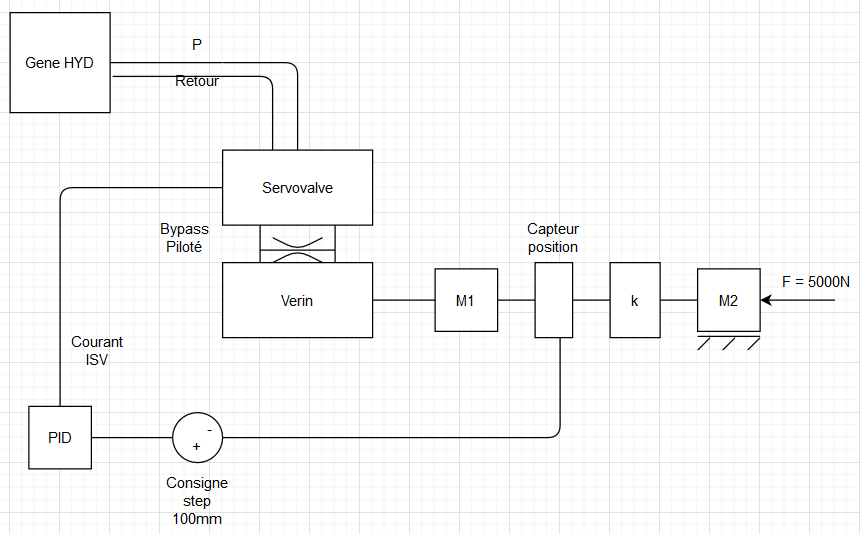
\includegraphics[width=\linewidth]{systeme1}
	\caption{Système hydrau-mécanique à modéliser}
\end{figure}
\clearpage
Les grandeurs de notre système sont pour la partie hydraulique : 
\begin{itemize}
	\item $P_{service} = 207$ bars (Pression standard de service dans un avion non A380)
	\item Bande passante servo valve: $50Hz$
	\item $I_{sv} = \pm 10mA$ (Finesse de la servo valve)
	\item $\Delta P = 35$ bars par orifice
	\item Course vérin : $300$ m 
	\item $F_{verin} = 10\ 000$ N 
	\item $v_{verin} = 150$ mm/s 
\end{itemize}


Pour la partie mécanique, les grandeurs sont :

\begin{itemize}
\item  $k=1.3\times 10^6$ N/m
\item  $m_1 = 10$ kg
\item $m_2 = 150$ kg
\item $f = 10$ N/(m/s)
\end{itemize}

\section{Détermination de paramètres supplémentaires}
\qquad Lors de la modélisation sur Amesim de notre système, nous aurons besoin de $3$ autres grandeurs qui nous permettront de paramétrer correctement notre simulation. Ceux-ci sont :
\begin{enumerate}
	\item $Q_n$ le débit nominal au niveau de la servo valve
	\item $D$ le diamètre du piston
	\item $d$ le diamètre de la tige
\end{enumerate}
Ces grandeurs sont reliées par une autre que l'on devra également calculer, qui est la surface d'action du vérin. On suppose pour des raisons de dimensionnement et de cohérence que $D = 3\times d$ Nous avons donc :
\begin{equation}
	S = S_{piston} - S_{tige} = \frac{\pi D^2}{4} - \frac{\pi d^2}{4} = \frac{\pi}{4} \times 8d^2 = 2\pi d
\end{equation}
D'où : 
\begin{align}
	d &= \sqrt{\frac{S}{2\pi}}\\
	D &= 3\sqrt{\frac{S}{2\pi}}
\end{align}
On commence par calculer la surface : 
\begin{equation}
	S = \frac{F}{P} = \frac{10\ 000N}{207\times 10^5\ Pa} = 4.83092\times 10^{-4} m^2
\end{equation}
D'où : 
\begin{align}
	d &= \sqrt{\frac{S}{2\pi}} = 8.7685\ mm\\
	D &= 3\sqrt{\frac{S}{2\pi}} = 26.3055\ mm\\
	Q_n &= S\times v = 0.15\times S = 7.2464\times 10^{-5}\ m^3/s = 4.34784\ L/min
\end{align}
Ces calculs sont fait en régime permanent, en statique, c'est pour cela que l'on considère une pression de $207$ bars.
\section{Modélisation et simulation dans Amesim}
\subsection{Blocs utilisés}
\begin{itemize}
	\itemsep0em
	\item Génératrice de pression (207 bars) (Hydraulique, Sources)
	\item Servo valve, quatre ports fermés (Hydraulique, Command valves extended)
	\item By-pass piloté, électrovalve (Hydraulique, Command valves)
	\item Vérin (Hydraulique, Linear actuators)
	\item Masse sans friction (Mécanique, Translation)
	\item Capteur de position (Mécanique, Translation)
	\item Ressort (Mécanique, Translation)
	\item Masse avec friction (Mécanique, Translation)
	\item Jonction de comparaison/différentiation (Signal, Maths)
	\item PID (Signal, Continuous)
\end{itemize}
\clearpage
La modélisation du système sous Amesim est donc : 
\begin{figure}[H]
	\centering 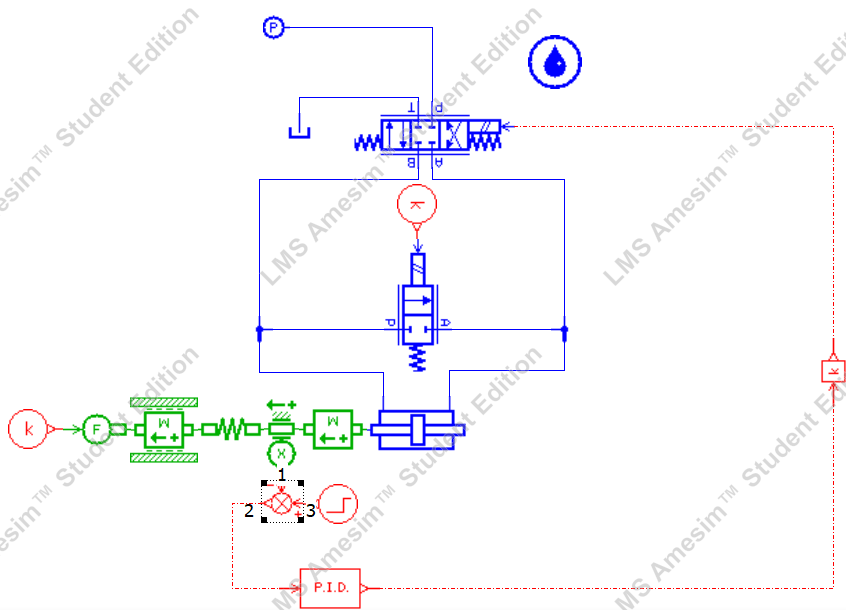
\includegraphics[width=\linewidth]{systemamesim}
	\caption{Modélisation sur Amesim}
\end{figure}
Le gain ajouté à la sortie du PID a une valeur de $-1$ et a été placé car la commande était opposée au step voulu. 
\clearpage
\subsection{Paramétrage}
Les paramètres obtenus par calcul précédemment sont en \textbf{gras}. Les valeurs non mentionnées dans ces tableaux sont celles définies par défaut par Amesim.
\subsubsection{Génératrice de pression}
On choisit pour la génératrice de pression de n'avoir qu'un seul stage, on ne souhaite pas avoir des paliers et souhaitons représenter l'actionneur dans un régime permanent où la pression est déjà au niveau de la pression opérationnelle standard d'un avion à $P = 207$ bars. 
\begin{table}[H]
	\centering
	\begin{tabular}{|c|c|c|}
		\hline
		\cellcolor{gray!30}Paramètre & \cellcolor{gray!30}Valeur & \cellcolor{gray!30}Unité\\
		\hline
		Number of stages & 1 & -\\
		\hline
		Pressure start of S1 & 207 & bars\\
		\hline 
		Pressure end of S1 & 207 & bars\\
		\hline
		Duration of S1 & 1e6 & seconds\\
		\hline
	\end{tabular}
\caption{Paramètrage de la génératrice de pression}
\end{table}
\subsubsection{Servo valve}
\begin{table}[H]
	\centering
	\begin{tabular}{|l|c|c|}
		\hline
		\cellcolor{gray!30}Paramètre & \cellcolor{gray!30}Valeur & \cellcolor{gray!30}Unité\\
		\hline
		\multicolumn{3}{c}{\cellcolor{green!30}Valve characteristics} \\
		\hline
		Valve rated current & 10 & mA\\
		\hline 
		Valve natural frequency & 50 & Hz\\
		\hline
		Duration of S1 & 1$\times$ 10$^6$ & seconds\\
		\hline
		\multicolumn{3}{c}{\cellcolor{green!30}Pressure drops and flow rates} \\
		\hline
		P to A flow rate at max opening & \textbf{4.34784} & L/min\\
		\hline
		P to A corresponding pressure drop & 35 & bars\\
		\hline
		B to T flow rate at max opening & \textbf{4.34784} & L/min\\
		\hline
		P to A corresponding pressure drop & 35 & bars\\
		\hline
		P to B flow rate at max opening & \textbf{4.34784} & L/min\\
		\hline
		P to A corresponding pressure drop & 35 & bars\\
		\hline
		A to T flow rate at max opening & \textbf{4.34784} & L/min\\
		\hline
		P to A corresponding pressure drop & 35 & bars\\
		\hline
	\end{tabular}
\caption{Paramètrage de la servo valve}
\end{table}
\subsubsection{By-pass piloté}
Pour le by-pass piloté, on utilise une électrovalve pilotée par un signal en entrée. Par exemple, on peut utiliser la valve02 qui est fermée lors que le signal de commande est à $k=0$ (fonctionnement normal) et est ouverte lorsque ce signal est à $k=1$. La valeur de ce signal est à paramétrer dans le signal constant $k$ sur le port $3$ du by-pass.
\begin{table}[H]
	\centering
	\begin{tabular}{|c|c|c|}
		\hline
		\cellcolor{gray!30}Paramètre & \cellcolor{gray!30}Valeur & \cellcolor{gray!30}Unité\\
		\hline
		\multicolumn{3}{c}{\cellcolor{green!30}Valve} \\
		\hline
		Valve natural frequency & 50 & Hz\\
		\hline
		\multicolumn{3}{c}{\cellcolor{green!30}Valve control} \\
		\hline
		Control signal value & 0/1 & -\\
		\hline
	\end{tabular}
	\caption{Paramètrage du by pass}
\end{table}
\subsubsection{Vérin}

\begin{table}[H]
	\centering
	\begin{tabular}{|c|c|c|}
		\hline
		\cellcolor{gray!30}Paramètre & \cellcolor{gray!30}Valeur & \cellcolor{gray!30}Unité\\
		\hline
		Piston diameter & \textbf{26.3055} & mm\\
		\hline
		Rod diameter at port 1 end & \textbf{8.7685} & mm\\
		\hline
		Rod diameter at port 2 end & \textbf{8.7685} & mm\\
		\hline
		Length of stroke (course) & 300 & mm\\
		\hline
	\end{tabular}
	\caption{Paramètrage du vérin}
\end{table}
\subsubsection{Première masse}
La première masse est celle entre le vérin et le capteur.
\begin{table}[H]
	\centering
	\begin{tabular}{|c|c|c|}
		\hline
		\cellcolor{gray!30}Paramètre & \cellcolor{gray!30}Valeur & \cellcolor{gray!30}Unité\\
		\hline
		Mass & 10 & kg\\
		\hline
	\end{tabular}
	\caption{Paramètrage de la première masse}
\end{table}
\subsubsection{Ressort}

\begin{table}[H]
	\centering
	\begin{tabular}{|c|c|c|}
		\hline
		\cellcolor{gray!30}Paramètre & \cellcolor{gray!30}Valeur & \cellcolor{gray!30}Unité\\
		\hline
		Spring rate (raideur) & 1.3 $\times$ 10$^6$ & kg\\
		\hline
	\end{tabular}
	\caption{Paramètrage du ressort}
\end{table}
\subsubsection{Deuxième masse}
La deuxième masse est celle qui subit une force et est reliée au ressort. Elle est également soumise à une friction.
\begin{table}[H]
	\centering
	\begin{tabular}{|c|c|c|}
		\hline
		\cellcolor{gray!30}Paramètre & \cellcolor{gray!30}Valeur & \cellcolor{gray!30}Unité\\
		\hline
		\multicolumn{3}{c}{\cellcolor{green!30}Mass} \\
		\hline
		Mass & 150 & kg\\
		\hline
		Coefficient of viscous friction & 10 & N/(m/s)\\
		\hline
		\multicolumn{3}{c}{\cellcolor{green!30}Force applied to the mass} \\
		\hline
		Value of $k$ signal & 5000 & - (defined as Newton in the force block)\\
		\hline
	\end{tabular}
	\caption{Paramètrage de la deuxième masse}
\end{table}
\subsubsection{Commande}
Pour l'objectif visé, on utilise un step en entrée du PID avec : 
\begin{table}[H]
	\centering
	\begin{tabular}{|c|c|c|}
		\hline
		\cellcolor{gray!30}Paramètre & \cellcolor{gray!30}Valeur & \cellcolor{gray!30}Unité\\
		\hline
	    Value after step & 0.1 & - (physiquement, des $m$)\\
		\hline
		Step time & 2 & s\\
		\hline
	\end{tabular}
	\caption{Paramètrage du step}
\end{table}
\subsubsection{PID}
Les paramètres du PID ont été obtenus par tâtonnements en réglant tout d'abord la partie proportionnelle avec le reste à 0 puis, en réglant le paramètre intégral avec la partie proportionnelle fixée. Cela permet d'avoir tout d'abord un bon rise time pour approcher de la valeur souhaitée rapidement puis de réduire l'erreur en steady state, le tout sans avoir un trop grand overshoot.\\

On évite le coefficient dérivatif car celui-ci n'est pas nécessaire ici, on préfère utiliser un filtre dérivatif lorsque c'est réellement nécessaire.
\begin{table}[H]
	\centering
	\begin{tabular}{|c|c|c|}
		\hline
		\cellcolor{gray!30}Paramètre & \cellcolor{gray!30}Valeur & \cellcolor{gray!30}Unité\\
		\hline
		Proportional gain & 50 & - \\
		\hline
		Integral gain & 0.2 & -\\
		\hline
	\end{tabular}
	\caption{Paramètrage du PID}
\end{table}
\subsection{Simulation}
L'objectif de la simulation et du système est d'avoir un mouvement détecté par le capteur et que ce mouvement corresponde à une commande que l'on définit. On a ici choisi d'avoir un step à $100$ mm soit $0.1$ m. Pour des raisons de lisibilité on a choisi de mettre le step time à 2 secondes.\\

Le contrôle est effectué par un PID dont les paramètres sont réglés en fixant d'abord la partie proportionnelle puis la partie intégrale pour éliminer l'erreur en régime permanent. \\

En utilisant tous les paramètres cités auparavant, nous avons le graph suivant :
\begin{figure}[H]
	\centering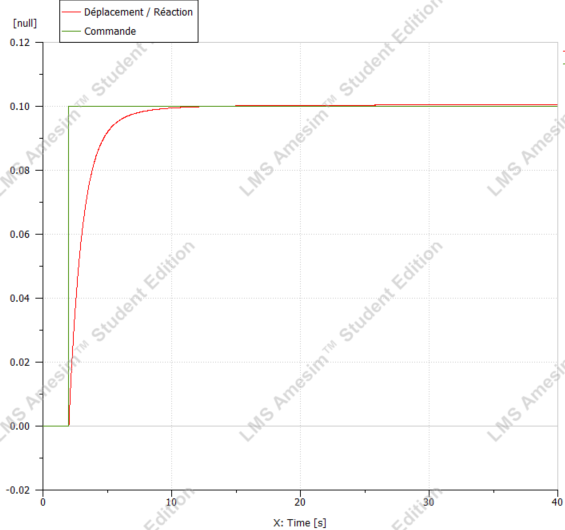
\includegraphics[width=\linewidth]{graph}
	\caption{Réaction du système à la commande}
\end{figure}

On voit sur ce graphique que le temps de convergence est environ de 12 secondes et, d'après les résultats de la simulation, la valeur finale du déplacement est de $0.10042$ m soit une erreur de régime permanent de $0.42\%$.
\section{Conclusion}
Plusieurs difficultées ont été rencontrées dans cette simulation. Celles-ci venaient principalement de fait que l'outil utilisé m'est nouveau. Le choix des blocs et les paramétrages pour certains éléments (servo valve et vérin) ont été assez difficiles étant donné la grande plage de paramètres disponibles.\\

La première difficulté est apparue lors du choix pour le By-Pass piloté, pour lequel la valve02 a été choisie puisqu'elle permettait de controller le débit en tout ou rien via un signal en entrée. Ce signal en entrée est $0$ lorsque le By-Pass n'est pas actif et $1$ lorsqu'il l'est.\\

Ensuite, j'ignorais au départ que faire pour définir le fluide nécessaire à notre système, qui a ensuite été défini dans Amesim par l'élément "General Hydraulic Properties".\\

Dans le vérin, un déplacement initial du piston ($\#$ sur Amesim) a été défini lors du troubleshoot afin de limiter les problèmes d'oscillations et d'instabilité sur le déplacement détecté par le capteur. Cependant, après d'autres tests en ayant relancé Amesim, les oscillations sont réapparues avec la nouvelle condition initiale, c'est pour cela que cette valeur a ensuite été remise à sa valeur par défaut soit $0$ m au lieu des $0.15$ m fixé lors du troubleshoot.
\clearpage
\newgeometry{margin=2cm}
\section{Tableau global des paramètres}
\begin{table}[H]
	\centering
	\begin{tabular}{|c|c|c|}
		\hline
		\cellcolor{gray!30}Paramètre & \cellcolor{gray!30}Valeur & \cellcolor{gray!30}Unité\\
		\hline
		\multicolumn{3}{c}{\cellcolor{green!30}Génératrice de pression} \\
		\hline
		Number of stages & 1 & -\\
		\hline
		Pressure start of S1 & 207 & bars\\
		\hline 
		Pressure end of S1 & 207 & bars\\
		\hline
		Duration of S1 & 1e6 & seconds\\
		\hline
		\multicolumn{3}{c}{\cellcolor{green!30}Caractéristiques de la servo valve} \\
		\hline
		Valve rated current & 10 & mA\\
		\hline 
		Valve natural frequency & 50 & Hz\\
		\hline
		Duration of S1 & 1$\times$ 10$^6$ & seconds\\
		\hline
		\multicolumn{3}{c}{\cellcolor{green!30}Débits et pertes de charge de la servo valve} \\
		\hline
		P to A flow rate at max opening & \textbf{4.34784} & L/min\\
		\hline
		P to A corresponding pressure drop & 35 & bars\\
		\hline
		B to T flow rate at max opening & \textbf{4.34784} & L/min\\
		\hline
		P to A corresponding pressure drop & 35 & bars\\
		\hline
		P to B flow rate at max opening & \textbf{4.34784} & L/min\\
		\hline
		P to A corresponding pressure drop & 35 & bars\\
		\hline
		A to T flow rate at max opening & \textbf{4.34784} & L/min\\
		\hline
		P to A corresponding pressure drop & 35 & bars\\
		\hline
		\multicolumn{3}{c}{\cellcolor{green!30}Valve By-Pass} \\
		\hline
		Valve natural frequency & 50 & Hz\\
		\hline
		\multicolumn{3}{c}{\cellcolor{green!30}Pilotage du By-Pass} \\
		\hline
		Control signal value & 0/1 & -\\
		\hline
		\multicolumn{3}{c}{\cellcolor{green!30}Vérin} \\
		\hline
		Piston diameter & \textbf{26.3055} & mm\\
		\hline
		Rod diameter at port 1 end & \textbf{8.7685} & mm\\
		\hline
		Rod diameter at port 2 end & \textbf{8.7685} & mm\\
		\hline
		Length of stroke (course) & 300 & mm\\
		\hline
		\multicolumn{3}{c}{\cellcolor{green!30}Première masse}\\
		\hline
		Mass & 10 & kg\\
		\hline
		\multicolumn{3}{c}{\cellcolor{green!30}Ressort}\\
		\hline
		Spring rate (raideur) & 1.3 $\times$ 10$^6$ & kg\\
		\hline
		\multicolumn{3}{c}{\cellcolor{green!30}Deuxième masse} \\
		\hline
		Mass & 150 & kg\\
		\hline
		Coefficient of viscous friction & 10 & N/(m/s)\\
		\hline
		\multicolumn{3}{c}{\cellcolor{green!30}Force appliquée à la deuxième masse} \\
		\hline
		Value of $k$ signal & 5000 & - (defined as Newton in the force block)\\
		\hline
		\multicolumn{3}{c}{\cellcolor{green!30}Commande step} \\
		\hline
		Value after step & 0.1 & - (physiquement, des $m$)\\
		\hline
		Step time & 2 & s\\
		\hline
		\multicolumn{3}{c}{\cellcolor{green!30}PID} \\
		\hline
		Proportional gain & 50 & - \\
		\hline
		Integral gain & 0.2 & -\\
		\hline
	\end{tabular}
	\caption{Paramètrage global}
\end{table}
\clearpage
\chapter{Actionneur électrique}
\end{document}